% Options for packages loaded elsewhere
\PassOptionsToPackage{unicode}{hyperref}
\PassOptionsToPackage{hyphens}{url}
\PassOptionsToPackage{dvipsnames,svgnames,x11names}{xcolor}
%
\documentclass[
  letterpaper,
  DIV=11,
  numbers=noendperiod]{scrartcl}

\usepackage{amsmath,amssymb}
\usepackage{iftex}
\ifPDFTeX
  \usepackage[T1]{fontenc}
  \usepackage[utf8]{inputenc}
  \usepackage{textcomp} % provide euro and other symbols
\else % if luatex or xetex
  \usepackage{unicode-math}
  \defaultfontfeatures{Scale=MatchLowercase}
  \defaultfontfeatures[\rmfamily]{Ligatures=TeX,Scale=1}
\fi
\usepackage{lmodern}
\ifPDFTeX\else  
    % xetex/luatex font selection
\fi
% Use upquote if available, for straight quotes in verbatim environments
\IfFileExists{upquote.sty}{\usepackage{upquote}}{}
\IfFileExists{microtype.sty}{% use microtype if available
  \usepackage[]{microtype}
  \UseMicrotypeSet[protrusion]{basicmath} % disable protrusion for tt fonts
}{}
\makeatletter
\@ifundefined{KOMAClassName}{% if non-KOMA class
  \IfFileExists{parskip.sty}{%
    \usepackage{parskip}
  }{% else
    \setlength{\parindent}{0pt}
    \setlength{\parskip}{6pt plus 2pt minus 1pt}}
}{% if KOMA class
  \KOMAoptions{parskip=half}}
\makeatother
\usepackage{xcolor}
\setlength{\emergencystretch}{3em} % prevent overfull lines
\setcounter{secnumdepth}{5}
% Make \paragraph and \subparagraph free-standing
\ifx\paragraph\undefined\else
  \let\oldparagraph\paragraph
  \renewcommand{\paragraph}[1]{\oldparagraph{#1}\mbox{}}
\fi
\ifx\subparagraph\undefined\else
  \let\oldsubparagraph\subparagraph
  \renewcommand{\subparagraph}[1]{\oldsubparagraph{#1}\mbox{}}
\fi


\providecommand{\tightlist}{%
  \setlength{\itemsep}{0pt}\setlength{\parskip}{0pt}}\usepackage{longtable,booktabs,array}
\usepackage{calc} % for calculating minipage widths
% Correct order of tables after \paragraph or \subparagraph
\usepackage{etoolbox}
\makeatletter
\patchcmd\longtable{\par}{\if@noskipsec\mbox{}\fi\par}{}{}
\makeatother
% Allow footnotes in longtable head/foot
\IfFileExists{footnotehyper.sty}{\usepackage{footnotehyper}}{\usepackage{footnote}}
\makesavenoteenv{longtable}
\usepackage{graphicx}
\makeatletter
\def\maxwidth{\ifdim\Gin@nat@width>\linewidth\linewidth\else\Gin@nat@width\fi}
\def\maxheight{\ifdim\Gin@nat@height>\textheight\textheight\else\Gin@nat@height\fi}
\makeatother
% Scale images if necessary, so that they will not overflow the page
% margins by default, and it is still possible to overwrite the defaults
% using explicit options in \includegraphics[width, height, ...]{}
\setkeys{Gin}{width=\maxwidth,height=\maxheight,keepaspectratio}
% Set default figure placement to htbp
\makeatletter
\def\fps@figure{htbp}
\makeatother
% definitions for citeproc citations
\NewDocumentCommand\citeproctext{}{}
\NewDocumentCommand\citeproc{mm}{%
  \begingroup\def\citeproctext{#2}\cite{#1}\endgroup}
\makeatletter
 % allow citations to break across lines
 \let\@cite@ofmt\@firstofone
 % avoid brackets around text for \cite:
 \def\@biblabel#1{}
 \def\@cite#1#2{{#1\if@tempswa , #2\fi}}
\makeatother
\newlength{\cslhangindent}
\setlength{\cslhangindent}{1.5em}
\newlength{\csllabelwidth}
\setlength{\csllabelwidth}{3em}
\newenvironment{CSLReferences}[2] % #1 hanging-indent, #2 entry-spacing
 {\begin{list}{}{%
  \setlength{\itemindent}{0pt}
  \setlength{\leftmargin}{0pt}
  \setlength{\parsep}{0pt}
  % turn on hanging indent if param 1 is 1
  \ifodd #1
   \setlength{\leftmargin}{\cslhangindent}
   \setlength{\itemindent}{-1\cslhangindent}
  \fi
  % set entry spacing
  \setlength{\itemsep}{#2\baselineskip}}}
 {\end{list}}
\usepackage{calc}
\newcommand{\CSLBlock}[1]{\hfill\break\parbox[t]{\linewidth}{\strut\ignorespaces#1\strut}}
\newcommand{\CSLLeftMargin}[1]{\parbox[t]{\csllabelwidth}{\strut#1\strut}}
\newcommand{\CSLRightInline}[1]{\parbox[t]{\linewidth - \csllabelwidth}{\strut#1\strut}}
\newcommand{\CSLIndent}[1]{\hspace{\cslhangindent}#1}

\KOMAoption{captions}{tableheading}
\makeatletter
\@ifpackageloaded{caption}{}{\usepackage{caption}}
\AtBeginDocument{%
\ifdefined\contentsname
  \renewcommand*\contentsname{Table of contents}
\else
  \newcommand\contentsname{Table of contents}
\fi
\ifdefined\listfigurename
  \renewcommand*\listfigurename{List of Figures}
\else
  \newcommand\listfigurename{List of Figures}
\fi
\ifdefined\listtablename
  \renewcommand*\listtablename{List of Tables}
\else
  \newcommand\listtablename{List of Tables}
\fi
\ifdefined\figurename
  \renewcommand*\figurename{Figure}
\else
  \newcommand\figurename{Figure}
\fi
\ifdefined\tablename
  \renewcommand*\tablename{Table}
\else
  \newcommand\tablename{Table}
\fi
}
\@ifpackageloaded{float}{}{\usepackage{float}}
\floatstyle{ruled}
\@ifundefined{c@chapter}{\newfloat{codelisting}{h}{lop}}{\newfloat{codelisting}{h}{lop}[chapter]}
\floatname{codelisting}{Listing}
\newcommand*\listoflistings{\listof{codelisting}{List of Listings}}
\makeatother
\makeatletter
\makeatother
\makeatletter
\@ifpackageloaded{caption}{}{\usepackage{caption}}
\@ifpackageloaded{subcaption}{}{\usepackage{subcaption}}
\makeatother
\ifLuaTeX
  \usepackage{selnolig}  % disable illegal ligatures
\fi
\usepackage{bookmark}

\IfFileExists{xurl.sty}{\usepackage{xurl}}{} % add URL line breaks if available
\urlstyle{same} % disable monospaced font for URLs
\hypersetup{
  pdftitle={Temporal and spatial variations of PM2.5 and PM10 concentrations in Mongolia},
  pdfauthor={Erdenebayar Munkhtsetseg; Atsushi Shimizu},
  pdfkeywords={particulate matters, concentrations of PM10 and PM2.5},
  colorlinks=true,
  linkcolor={blue},
  filecolor={Maroon},
  citecolor={Blue},
  urlcolor={Blue},
  pdfcreator={LaTeX via pandoc}}

\title{Temporal and spatial variations of PM2.5 and PM10 concentrations
in Mongolia}
\author{Erdenebayar Munkhtsetseg \and Atsushi Shimizu}
\date{2024-03-16}

\begin{document}
\maketitle
\begin{abstract}
PM2.5 and PM10 data for the 4 distinct sites of Mongolia from 2008 to
2020 is found \ldots. \ldots{}
\end{abstract}

\section{Introduction}\label{introduction}

\section{Data \& Methods}\label{sec-data-methods}

\subsection{Study area descriptions}\label{study-area-descriptions}

Dust monitoring sites were located at Dalanzadgad (43.57°N, 104.42°E),
Sainshand (44.87°N, 110.12°E), Erdene (44.27°N, 111.05°E) and Zamyn-Uud
(43.72°N, 111.90°E) in the Gobi Desert, and at Bayan Unjuul (47.02°N,
105.56°E) in a steppe zone of Mon- golia (Fig. 1). Particulate matter
with aerodynamic diameters less than 2.5 lm (PM2.5) and 10 lm (PM10)
were measured at these sites using an instrument that measures light
scattering by air- borne particulates. Meteorological parameters,
including air tem- perature, precipitation, wind and visibility were
determined by automatic instruments and are detailed in previous
articles (Jugder et al., 2011, 2012; Kimura and Shinoda, 2010; Park et
al., 2010; Shinoda et al., 2010). The instruments for measuring
particulate matters were placed 2.0 m above the ground level (AGL) at
Dalanzadgad, Sainshand and Zamyn-Uud, at 3.0 m AGL at Erdene, and at 1.9
m AGL at Bayan Unjuul (Tables 1a--c). Wind sensors were installed at
3--4 m AGL at the four Gobi sites, and visibility (meteorological
optical range-MOR) sensors with a maximum measurement range of 20 km
were installed at a height of 3 m AGL at three of the sites, excluding
Erdene. At the Bayan Unjuul site, the wind sensor height used was 1.54 m
AGL, and a visibility sensor with a maximum measurement range of 2 km
was placed at 1.8 m AGL. Datasets were obtained from measurements at
Dalanzadgad, Sainshand, Erdene, and Zamyn-Uud from January 2009 to May
2013, and at Bayan Unjuul from the end of April to May 2008. The data
used in the study are based on hourly means derived from 1 and 10 min
averages. Additionally, the WMO defines dust storms and sandstorms (dust
events) as ``An ensemble of particles of dust and sand energetically
lifted to great heights by a strong and turbulent wind'' (WMO-No.~407)
and reducing visibility to less than 1000 m (WMO-No.~306). Therefore,
data of wind speed, visibility, and dust concentration were used in
combination with synoptic weather observations. Data sets comprise
selected data collections from periods of dust events, during which wind
speeds and PM10 (PM2.5) concentration rose dramatically and visibility
dropped down considerably. Quantitative criterion of wind speeds and
dust con- centrations of PM10 for dust events were explained in Section
2.2. Scalar mean wind speed and gust winds were calculated from 1-s
observations for the study (EPA-454/R-99-005, 2000). The shorter
averaging period wind is regarded as the ``gust'' (Harper et al., 2010).
The 3-s averages of wind speed that are considered as gust wind speed
(Harper et al., 2010), were used in this study. Time series of number of
days with dust events obtained from synoptic weather observations at
Dalanzadgad, Sainshand and Zamyn-Uud during 1960--2012 were used.

See Figure~\ref{fig-1} djjd

\begin{figure}

\centering{

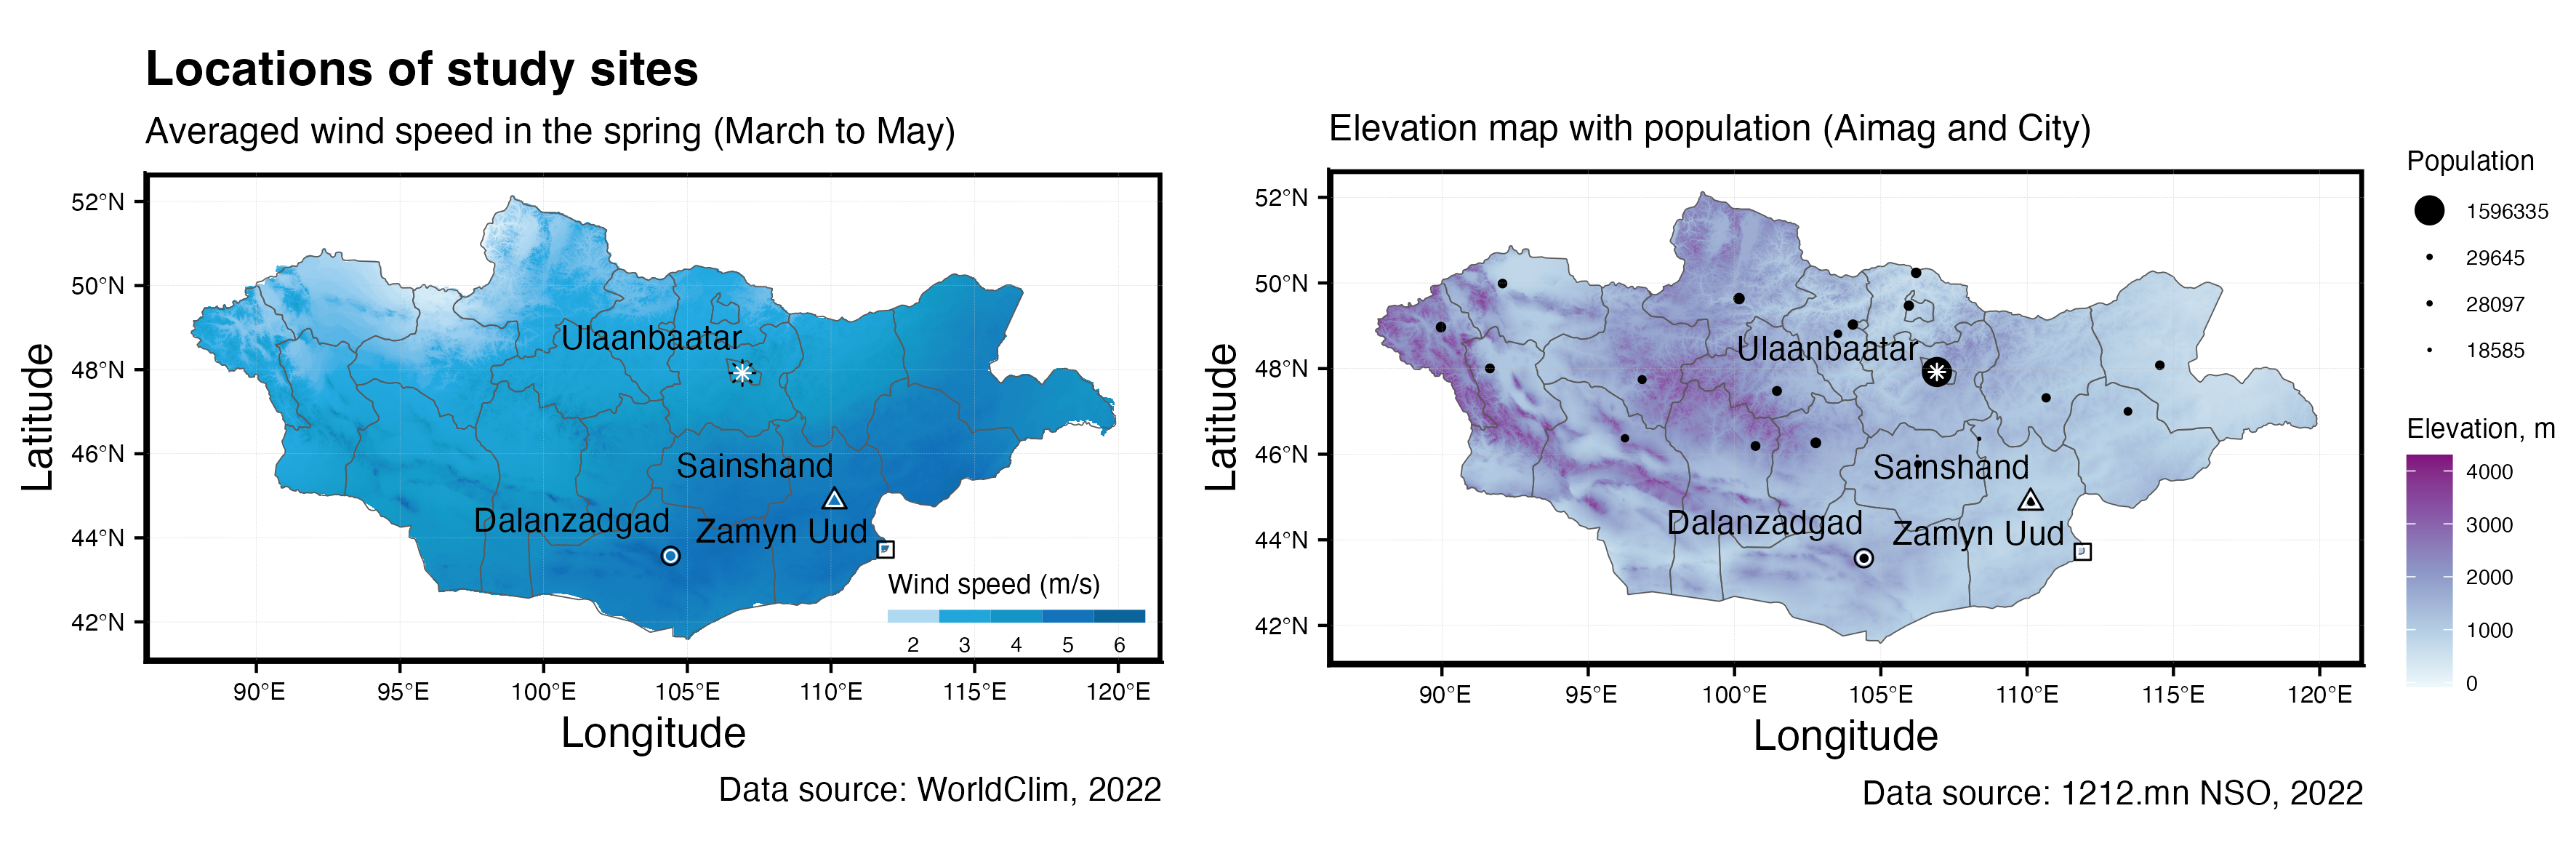
\includegraphics{../Data/03_figures/fig-1_sites_of_NIES.png}

}

\caption{\label{fig-1}Study sites}

\end{figure}%

The map demonstrates that llll

\subsection{Study data and data
analysis}\label{study-data-and-data-analysis}

\begin{table}

\caption{\label{tbl-1}Data}

\centering{

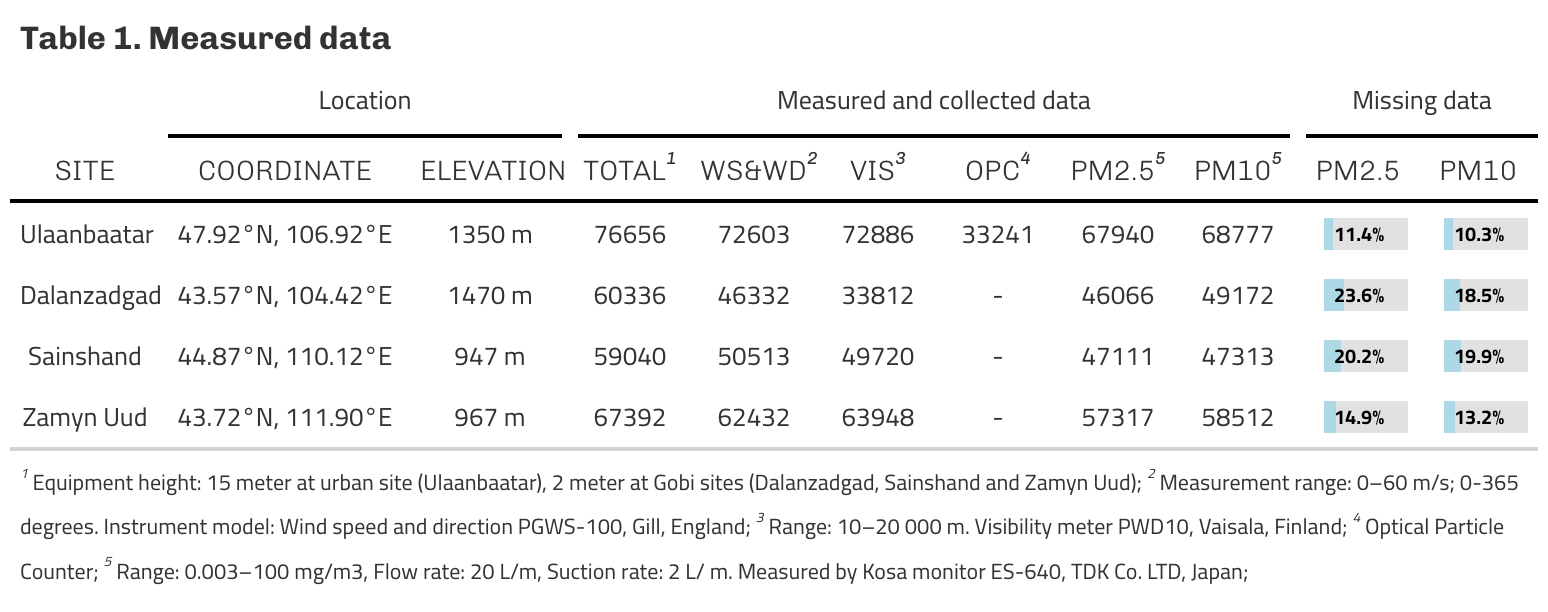
\includegraphics{../Data/03_tables/table-1_data_NIES.png}

}

\end{table}%

Table~\ref{tbl-1} djjdjdjjdj

a summarises the data. cleaned the data and filled the missing data
using mtsdi

\section{Results}\label{sec-results}

\section{Discussion}\label{sec-discussion}

\section{Conclusions}\label{sec-conclusions}

Marrero et al. (2019) \# References \{.unnumbered\}

\{\#refs\}

\phantomsection\label{refs}
\begin{CSLReferences}{1}{0}
\bibitem[\citeproctext]{ref-marrero2019}
Marrero, José, Alicia García, Manuel Berrocoso, Ángeles Llinares,
Antonio Rodríguez-Losada, and R. Ortiz. 2019. {``Strategies for the
Development of Volcanic Hazard Maps in Monogenetic Volcanic Fields: The
Example of {La} {Palma} ({Canary} {Islands}).''} \emph{Journal of
Applied Volcanology} 8 (July).
\url{https://doi.org/10.1186/s13617-019-0085-5}.

\end{CSLReferences}



\end{document}
